% IntelliSafe -- FYP-I Proposal Presentation (revised)
% Build: xelatex intellisafe_proposal.tex (run twice)
\documentclass[aspectratio=169,10pt]{beamer}

\usetheme[progressbar=none, numbering=fraction, sectionpage=none, block=fill]{metropolis}

\usepackage{booktabs}
\usepackage{tabularx}
\usepackage{array}
\usepackage{amssymb}
\usepackage{pifont}
\usepackage{pgfgantt}
\usepackage{tikz}
\usetikzlibrary{positioning, arrows.meta, shapes.geometric, shapes.misc, fit, backgrounds, calc}

% ---------- palette (matches the original deck) ----------
\definecolor{navy}{HTML}{1F3A5F}
\definecolor{teal}{HTML}{0E7C86}
\definecolor{amber}{HTML}{E8A33D}
\definecolor{crit}{HTML}{C0392B}
\definecolor{slate}{HTML}{5D6D7E}
\definecolor{leaf}{HTML}{2E7D4F}
\definecolor{paper}{HTML}{F4F6F8}

\setbeamercolor{frametitle}{bg=navy, fg=white}
\setbeamercolor{normal text}{fg=black!85, bg=white}
\setbeamercolor{alerted text}{fg=teal}
\setbeamercolor{example text}{fg=amber}
\setbeamercolor{block title}{bg=teal!15, fg=navy}
\setbeamercolor{block body}{bg=paper, fg=black!85}
\setbeamercolor{block title alerted}{bg=crit!15, fg=crit}
\setbeamercolor{block body alerted}{bg=paper, fg=black!85}
\setbeamercolor{progress bar}{fg=amber, bg=slate!30}
\setbeamertemplate{itemize item}{\color{teal}$\blacktriangleright$}
\setbeamertemplate{itemize subitem}{\color{slate}--}
\setbeamerfont{frametitle}{size=\large, series=\bfseries}

\newcommand{\yes}{\textcolor{leaf}{\ding{51}}}
\newcommand{\nr}{\textcolor{slate!60}{--}}
\newcommand{\prio}[2]{\colorbox{#1}{\textcolor{white}{\tiny\bfseries\strut #2}}}
\newcolumntype{L}[1]{>{\raggedright\arraybackslash}p{#1}}
\newcolumntype{C}[1]{>{\centering\arraybackslash}p{#1}}
\newcolumntype{Y}{>{\raggedright\arraybackslash}X}

\tikzset{
  blk/.style={draw=#1, fill=#1!10, rounded corners=2pt, align=center, font=\scriptsize,
              minimum height=0.8cm, minimum width=1.9cm, inner sep=2pt, line width=0.6pt},
  blk/.default=teal,
  arr/.style={-{Stealth[length=4pt]}, line width=0.6pt, draw=navy!85},
  arrc/.style={-{Stealth[length=4pt]}, line width=0.8pt, draw=crit},
  lbl/.style={font=\tiny, text=slate, fill=white, inner sep=1pt},
  grp/.style={draw=slate!55, dashed, rounded corners=4pt, inner sep=5pt},
  grpt/.style={font=\tiny\bfseries, text=slate, anchor=south west, inner sep=1pt},
  dec/.style={diamond, aspect=1.7, draw=amber, fill=amber!12, align=center, font=\tiny,
              inner sep=0.5pt, line width=0.6pt},
  term/.style={rounded rectangle, draw=leaf, fill=leaf!10, font=\scriptsize,
               minimum height=0.6cm, minimum width=1.4cm, line width=0.6pt},
  io/.style={trapezium, trapezium left angle=72, trapezium right angle=108, draw=teal,
             fill=teal!10, align=center, font=\scriptsize, minimum height=0.8cm, line width=0.6pt},
}

\title{IntelliSafe}
\subtitle{Real-Time Working Site Safety Monitoring using Edge Computer Vision}

\begin{document}

% =====================================================================
% 1. Title
% =====================================================================
\begin{frame}[plain]
  \centering
  \vspace{-0.3em}
  
\includegraphics[height=1.45cm]{comsats_logo.pdf}\par\vspace{0.25em}
  {\small\color{slate} COMSATS University Islamabad, Lahore Campus}\par
  {\footnotesize\color{slate} Department of Computer Engineering}\par\vspace{0.35em}
  {\scriptsize\bfseries\color{amber} FYP-I PROJECT PROPOSAL}\par\vspace{0.3em}
  {\LARGE\bfseries\color{navy} IntelliSafe}\par\vspace{0.15em}
  {\normalsize\color{navy} Real-Time Working Site Safety Monitoring using Edge Computer Vision}\par
  \vspace{0.35em}{\color{slate!50}\rule{0.55\linewidth}{0.4pt}}\par\vspace{0.3em}
  {\footnotesize
  \begin{tabular}{lll}
    \toprule
    \textbf{Group Member} & \textbf{Reg. ID} & \textbf{Email}\\
    \midrule
    Muhammad Ahmad & FA23-BCE-113 & \texttt{fa23-bce-113@cuilahore.edu.pk}\\
    Uzair          & FA23-BCE-098 & \texttt{fa23-bce-098@cuilahore.edu.pk}\\
    \bottomrule
  \end{tabular}}\par\vspace{0.35em}
  {\footnotesize\textbf{Project Supervisor:} Dr.\ Ikramullah Khosa}\par\vspace{0.15em}
  {\scriptsize\color{slate} Fall 2026}
\end{frame}

% =====================================================================
% 2. Outline
% =====================================================================
\begin{frame}{Outline}
  \begin{columns}[T]
    \begin{column}{0.48\textwidth}
      \begin{enumerate}
        \item Abstract
        \item Motivation \& Problem Statement
        \item Literature Review
        \item Research Gap \& Our Contribution
        \item Objectives \& Research Questions
        \item Deliverables \& SDG Mapping
      \end{enumerate}
    \end{column}
    \begin{column}{0.48\textwidth}
      \begin{enumerate}\setcounter{enumi}{6}
        \item Methodology: architecture, flow chart, model, compliance engine, emergency alarm, event pipeline
        \item Evaluation Plan
        \item Work Distribution \& Timeline
        \item Conclusion \& References
      \end{enumerate}
    \end{column}
  \end{columns}
\end{frame}

% =====================================================================
% 3. Abstract
% =====================================================================
\begin{frame}{Abstract}
  \begin{columns}[c]
    \begin{column}{0.60\textwidth}
      \small
      IntelliSafe is an edge-based safety monitoring system for industrial and construction sites.
      A camera on an \textbf{NVIDIA Jetson Nano} runs a single \textbf{YOLOv8n} detector for
      \emph{worker, helmet, vest, fire} and \emph{smoke}. A \textbf{compliance engine} links each
      helmet and vest to its worker, keeps a rolling compliance score, and raises \emph{one} alert
      per continuing violation with an image as evidence.

      \medskip
      Events travel over \textbf{MQTT} to a backend that stores them, streams them to a supervisor
      dashboard and produces PDF compliance reports. For fire or smoke, an \textbf{ESP32 alarm unit}
      sounds a buzzer on site (target: within one second), even if the internet link is down.
    \end{column}
    \begin{column}{0.36\textwidth}
      \centering
      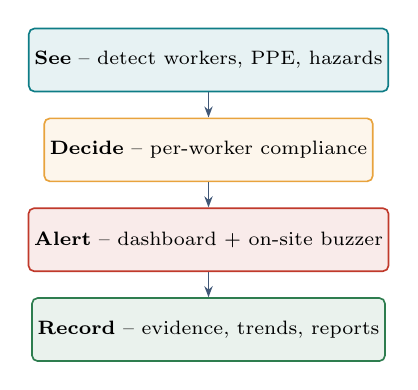
\begin{tikzpicture}[node distance=0.32cm]
        \node[blk=teal, minimum width=3.6cm] (a) {\textbf{See} -- detect workers, PPE, hazards};
        \node[blk=amber, minimum width=3.6cm, below=of a] (b) {\textbf{Decide} -- per-worker compliance};
        \node[blk=crit, minimum width=3.6cm, below=of b] (c) {\textbf{Alert} -- dashboard + on-site buzzer};
        \node[blk=leaf, minimum width=3.6cm, below=of c] (d) {\textbf{Record} -- evidence, trends, reports};
        \draw[arr] (a) -- (b); \draw[arr] (b) -- (c); \draw[arr] (c) -- (d);
      \end{tikzpicture}
    \end{column}
  \end{columns}
\end{frame}

% =====================================================================
% 4. Motivation & Problem
% =====================================================================
\begin{frame}{Motivation \& Problem Statement}
  \begin{columns}[T]
    \begin{column}{0.52\textwidth}
      \textbf{\small Why it matters}
      \begin{itemize}\footnotesize
        \item ILO: \alert{$\approx$\,3 million} work-related deaths and \alert{395~million}
              non-fatal injuries per year~[1].
        \item Construction and manufacturing carry a large share; missing PPE and unnoticed fire or
              smoke are recurring causes.
      \end{itemize}
      \vspace{0.2em}
      \textbf{\small Why current practice fails}
      \begin{itemize}\footnotesize
        \item \textbf{Coverage gaps} -- periodic rounds miss violations in between.
        \item \textbf{Human limits} -- one supervisor cannot watch every worker all shift.
        \item \textbf{No evidence} -- incidents are rebuilt from memory.
        \item \textbf{No trends} -- nobody knows which zone or shift is the weak point.
      \end{itemize}
    \end{column}
    \begin{column}{0.44\textwidth}
      \begin{block}{Problem statement}
        \small Design and implement a \textbf{low-cost edge computer-vision platform} that monitors a
        work site in real time, detects PPE non-compliance and fire or smoke, and delivers
        \textbf{alerts, on-site alarms, image evidence} and \textbf{compliance analytics} to
        supervisors.
      \end{block}
      \vspace{0.3em}
      {\scriptsize\color{slate} Approved detection scope: worker, helmet, vest, fire, smoke.\par}
    \end{column}
  \end{columns}
\end{frame}

% =====================================================================
% 5. Literature Review
% =====================================================================
\begin{frame}{Literature Review -- Prior Work}
  \scriptsize
  \renewcommand{\arraystretch}{1.25}
  \begin{tabularx}{\linewidth}{@{}L{2.0cm} L{3.0cm} L{2.4cm} L{2.4cm} Y@{}}
    \toprule
    \textbf{Work} & \textbf{Method} & \textbf{Data / Platform} & \textbf{Reported result} & \textbf{Open issue for a real site}\\
    \midrule
    \textbf{Nath et al.}~[2] \newline {\tiny Autom.\ Constr.\ 2020}
      & YOLOv3, three approaches; best one detects a worker and classifies PPE state (none / hat / vest / both)
      & Pictor-v3, $\sim$1.5k images; laptop
      & \textbf{72.3\% mAP} at 11 FPS
      & Image-level verdict; no hazards, no alerting, evidence or trends\\
    \textbf{Wang et al.}~[3] \newline {\tiny Sensors 2021}
      & Eight YOLO v3/v4/v5 detectors compared
      & CHV, 1,330 images, 6 classes; Tesla P40 GPU, PC / cloud
      & YOLOv5x \textbf{86.55\% mAP}; YOLOv5s \textbf{52 FPS}
      & Detects PPE items only; no worker-level decision; server GPU\\
    \textbf{de Ven\^ancio et al.}~[7] \newline {\tiny Neural Comput.\ Appl.\ 2022}
      & YOLOv4 fire/smoke detector + filter pruning
      & D-Fire, 21k+ images; Raspberry Pi 4
      & Up to \textbf{83.6\%} less compute, \textbf{83.9\%} less memory, no accuracy loss
      & Fire only; no PPE, no alert delivery or dashboard\\
    \bottomrule
  \end{tabularx}\par\vspace{0.2em}
  {\tiny\color{slate} Detector basis: YOLO single-pass detection~[4] and its current release,
  Ultralytics YOLOv8~[5], whose nano variant we deploy.\par}

  \vspace{0.6em}
  {\small\textbf{Takeaway.} Detection of PPE~[2,\,3] and fire~[7] is solved well enough to build on.
  What these works leave open is the \emph{system around the detector}.\par}
\end{frame}

% =====================================================================
% 6. Research Gap & Contribution
% =====================================================================
\begin{frame}{Research Gap \& Our Contribution -- How IntelliSafe Differs}
  \begin{columns}[T]
    \begin{column}{0.53\textwidth}
      \scriptsize
      \renewcommand{\arraystretch}{1.12}
      \begin{tabular}{@{}l C{0.45cm} C{0.45cm} C{0.45cm} C{1.3cm}@{}}
        \toprule
        \textbf{Capability} & [2] & [3] & [7] & \textbf{\color{teal}IntelliSafe}\\
        \midrule
        Helmet + vest detection         & \yes & \yes & \nr  & \yes\\
        Fire / smoke detection          & \nr  & \nr  & \yes & \yes\\
        PPE + hazards in \emph{one} model & \nr & \nr & \nr  & \yes\\
        Worker-level compliance verdict & \yes & \nr  & \nr  & \yes\\
        Temporal debounce, priorities   & \nr  & \nr  & \nr  & \yes\\
        Embedded / edge inference       & \nr  & \nr  & \yes & \yes\\
        Event delivery (MQTT)           & \nr  & \nr  & \nr  & \yes\\
        Image evidence + history        & \nr  & \nr  & \nr  & \yes\\
        Dashboard, trends, PDF reports  & \nr  & \nr  & \nr  & \yes\\
        On-site audible alarm (ESP32)   & \nr  & \nr  & \nr  & \yes\\
        \bottomrule
      \end{tabular}\par\vspace{0.2em}
      {\tiny\color{slate}\yes\ addressed in the paper \quad -- not reported in the paper}
    \end{column}
    \begin{column}{0.43\textwidth}
      \begin{block}{Contributions of this FYP}
        \scriptsize
        \begin{enumerate}
          \item \textbf{Unified 5-class edge detector} for PPE and hazards on a Jetson Nano.
          \item \textbf{Compliance engine}: IoU matching, rolling score, $N$-frame debounce and
                priority levels.
          \item \textbf{End-to-end event pipeline}: MQTT, storage, evidence, live dashboard and
                reports.
          \item \textbf{Local emergency alarm}: ESP32 buzzer for fire and smoke.
          \item \textbf{On-device evaluation}: mAP, FPS, latency and false alerts per hour.
        \end{enumerate}
      \end{block}
      \vspace{0.2em}
      {\scriptsize We do \emph{not} claim a new detector. The contribution is a deployable,
      measured system.\par}
    \end{column}
  \end{columns}
\end{frame}

% =====================================================================
% 7. Objectives & Research Questions
% =====================================================================
\begin{frame}{Objectives \& Research Questions}
  \begin{columns}[T]
    \begin{column}{0.55\textwidth}
      \textbf{\small Objectives}
      \begin{enumerate}\small
        \item \textbf{Detect} worker, helmet, vest, fire and smoke with YOLOv8n.
        \item \textbf{Decide} per-worker compliance, one alert per violation, with evidence.
        \item \textbf{Deploy} detector and engine in real time on the Jetson Nano.
        \item \textbf{Deliver} events over MQTT; sound an \textbf{ESP32 buzzer} on fire or smoke.
        \item \textbf{Store} events, compliance history and evidence images.
        \item \textbf{Present} live alerts, trends and PDF reports on a dashboard.
      \end{enumerate}
    \end{column}
    \begin{column}{0.41\textwidth}
      \begin{block}{Research questions}
        \scriptsize
        \textbf{RQ1.} Can one YOLOv8n model on a Jetson Nano detect all five classes in real time
        with mAP@0.5 $\geq$ 0.70?\par\smallskip
        \textbf{RQ2.} How much does $N$-frame debouncing cut false alerts per hour compared with
        frame-level alerting?\par\smallskip
        \textbf{RQ3.} What end-to-end latency is achieved from camera to dashboard and from camera
        to buzzer?
      \end{block}
    \end{column}
  \end{columns}
\end{frame}

% =====================================================================
% 8. Deliverables & SDGs
% =====================================================================
\begin{frame}{Deliverables \& SDG Mapping}
  \begin{columns}[T]
    \begin{column}{0.52\textwidth}
      \textbf{\small Deliverables at the end of FYP}
      \begin{enumerate}\small
        \item Annotated dataset and trained YOLOv8n model (5 classes).
        \item Jetson Nano application: detection, compliance engine, evidence.
        \item ESP32 alarm unit: buzzer and strobe, driven over MQTT.
        \item Backend with database for events, history and evidence.
        \item Web dashboard with live alerts, trends and PDF reports.
        \item FYP report, documentation and a live end-to-end demo.
      \end{enumerate}
    \end{column}
    \begin{column}{0.44\textwidth}
      \scriptsize
      \renewcommand{\arraystretch}{1.35}
      \begin{tabular}{@{}L{1.3cm} L{4.2cm}@{}}
        \toprule
        \textbf{SDG} & \textbf{How IntelliSafe contributes}\\
        \midrule
        \prio{leaf}{SDG 3} & Early PPE and fire/smoke detection prevents injuries.\\
        \prio{crit}{SDG 8} & Continuous monitoring supports safe, decent work.\\
        \prio{amber}{SDG 9} & Low-cost edge AI brings evidence-based safety to industry.\\
        \bottomrule
      \end{tabular}
    \end{column}
  \end{columns}
\end{frame}

% =====================================================================
% 9. System Architecture
% =====================================================================
\begin{frame}{Methodology -- System Architecture}
  \centering
  \resizebox{\linewidth}{!}{%
  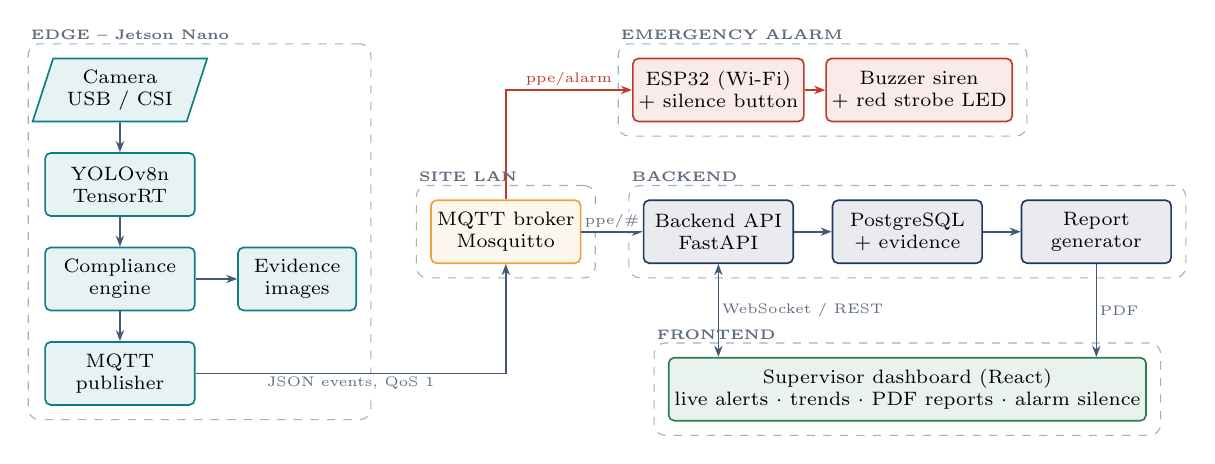
\begin{tikzpicture}
    % edge
    \node[io]          (cam)  at (0, 2.3)  {Camera\\USB / CSI};
    \node[blk=teal]    (yolo) at (0, 1.1)  {YOLOv8n\\TensorRT};
    \node[blk=teal]    (comp) at (0,-0.1)  {Compliance\\engine};
    \node[blk=teal]    (pub)  at (0,-1.3)  {MQTT\\publisher};
    \node[blk=teal, minimum width=1.5cm] (evid) at (2.25,-0.1) {Evidence\\images};
    % messaging
    \node[blk=amber]   (brk)  at (4.9, 0.5) {MQTT broker\\Mosquitto};
    % alarm
    \node[blk=crit]    (esp)  at (7.6, 2.3) {ESP32 (Wi-Fi)\\+ silence button};
    \node[blk=crit, minimum width=2.2cm] (bz) at (10.15, 2.3) {Buzzer siren\\+ red strobe LED};
    % backend
    \node[blk=navy]    (api)  at (7.6, 0.5) {Backend API\\FastAPI};
    \node[blk=navy]    (db)   at (10.0, 0.5) {PostgreSQL\\+ evidence};
    \node[blk=navy]    (rep)  at (12.4, 0.5) {Report\\generator};
    % frontend
    \node[blk=leaf, minimum width=5.7cm] (dash) at (10.0,-1.5)
         {Supervisor dashboard (React)\\live alerts $\cdot$ trends $\cdot$ PDF reports $\cdot$ alarm silence};

    \draw[arr] (cam) -- (yolo);
    \draw[arr] (yolo) -- (comp);
    \draw[arr] (comp) -- (pub);
    \draw[arr] (comp) -- (evid);
    \draw[arr] (pub.east) -| node[lbl, pos=0.25, below] {JSON events, QoS 1} (brk.south);
    \draw[arrc] (brk.north) |- node[lbl, pos=0.75, above] {\textcolor{crit}{ppe/alarm}} (esp.west);
    \draw[arrc] (esp) -- (bz);
    \draw[arr] (brk) -- node[lbl, above] {ppe/\#} (api);
    \draw[arr] (api) -- (db);
    \draw[arr] (db) -- (rep);
    \draw[arr, {Stealth[length=4pt]}-{Stealth[length=4pt]}] (api.south) -- node[lbl, right] {WebSocket / REST} (api.south |- dash.north);
    \draw[arr] (rep.south) -- node[lbl, right] {PDF} (rep.south |- dash.north);

    \begin{scope}[on background layer]
      \node[grp, fit=(cam)(pub)(evid)] (gE) {};
      \node[grp, fit=(brk)] (gM) {};
      \node[grp, fit=(esp)(bz)] (gA) {};
      \node[grp, fit=(api)(db)(rep)] (gB) {};
      \node[grp, fit=(dash)] (gF) {};
    \end{scope}
    \node[grpt] at (gE.north west) {EDGE -- Jetson Nano};
    \node[grpt] at (gM.north west) {SITE LAN};
    \node[grpt] at (gA.north west) {EMERGENCY ALARM};
    \node[grpt] at (gB.north west) {BACKEND};
    \node[grpt] at (gF.north west) {FRONTEND};
  \end{tikzpicture}}

  \vspace{0.3em}
  {\scriptsize\color{slate} The broker runs on the site LAN, so the buzzer still sounds if the backend
  or internet link is down. Event format is fixed up front, so model and platform work proceed in
  parallel; a simulator feeds the backend until the Jetson is ready.\par}
\end{frame}

% =====================================================================
% 10. Flow chart
% =====================================================================
\begin{frame}{Methodology -- Flow Chart}
  \centering
  \resizebox{\linewidth}{!}{%
  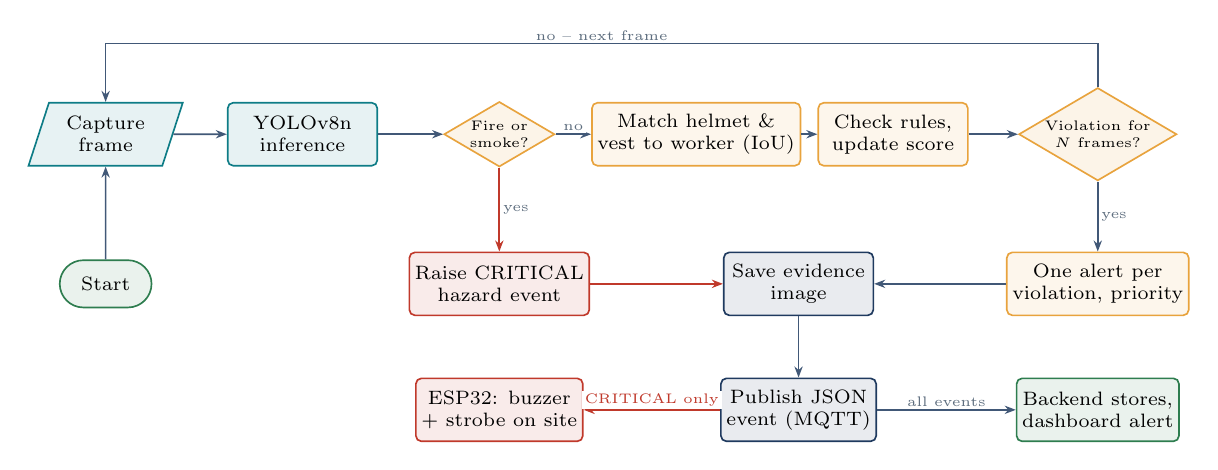
\begin{tikzpicture}
    % row A
    \node[io]        (cap)   at (0, 0)    {Capture\\frame};
    \node[blk=teal]  (yolo)  at (2.5, 0)  {YOLOv8n\\inference};
    \node[dec]       (d1)    at (5.0, 0)  {Fire or\\smoke?};
    \node[blk=amber] (iou)   at (7.5, 0)  {Match helmet \&\\vest to worker (IoU)};
    \node[blk=amber] (score) at (10.0, 0) {Check rules,\\update score};
    \node[dec]       (d2)    at (12.6, 0) {Violation for\\$N$ frames?};
    % row B
    \node[term]      (start) at (0,-1.9)  {Start};
    \node[blk=crit]  (crit)  at (5.0,-1.9){Raise CRITICAL\\hazard event};
    \node[blk=navy]  (evid)  at (8.8,-1.9){Save evidence\\image};
    \node[blk=amber] (alert) at (12.6,-1.9){One alert per\\violation, priority};
    % row C
    \node[blk=crit]  (esp)   at (5.0,-3.5){ESP32: buzzer\\+ strobe on site};
    \node[blk=navy]  (pub)   at (8.8,-3.5){Publish JSON\\event (MQTT)};
    \node[blk=leaf]  (back)  at (12.6,-3.5){Backend stores,\\dashboard alert};

    \draw[arr] (start) -- (cap);
    \draw[arr] (cap) -- (yolo);
    \draw[arr] (yolo) -- (d1);
    \draw[arr] (d1) -- node[lbl, above] {no} (iou);
    \draw[arr] (iou) -- (score);
    \draw[arr] (score) -- (d2);
    \draw[arr] (d2.north) -- ++(0,0.55) -| node[lbl, pos=0.25, above] {no -- next frame} (cap.north);
    \draw[arrc] (d1) -- node[lbl, right] {yes} (crit);
    \draw[arr] (d2) -- node[lbl, right] {yes} (alert);
    \draw[arrc] (crit) -- (evid);
    \draw[arr] (alert) -- (evid);
    \draw[arr] (evid) -- (pub);
    \draw[arrc] (pub) -- node[lbl, above] {\textcolor{crit}{CRITICAL only}} (esp);
    \draw[arr] (pub) -- node[lbl, above] {all events} (back);
  \end{tikzpicture}}

  \vspace{0.4em}
  {\scriptsize
  \tikz\node[blk=crit, minimum width=0.35cm, minimum height=0.22cm]{}; hazard path \quad
  \tikz\node[blk=amber, minimum width=0.35cm, minimum height=0.22cm]{}; PPE compliance path \quad
  \tikz\node[blk=navy, minimum width=0.35cm, minimum height=0.22cm]{}; evidence \& delivery\par
  \vspace{0.2em}{\color{slate} The edge loop runs every frame; the backend and alarm unit react asynchronously.}\par}
\end{frame}

% =====================================================================
% 11. Detection model
% =====================================================================
\begin{frame}{Methodology -- Detection Model \& Dataset}
  \begin{columns}[T]
    \begin{column}{0.48\textwidth}
      \small\textbf{One model, three detection tracks}\par\vspace{0.3em}
      \scriptsize
      \renewcommand{\arraystretch}{1.2}
      \begin{tabular}{@{}lll@{}}
        \toprule
        \textbf{Track} & \textbf{Class} & \textbf{Used for}\\
        \midrule
        Worker & worker & Anchor for the PPE check, tracking\\
        PPE    & helmet & Violation: \texttt{helmet\_missing}\\
        PPE    & vest   & Violation: \texttt{vest\_missing}\\
        Hazard & fire   & CRITICAL event + buzzer\\
        Hazard & smoke  & CRITICAL event + buzzer\\
        \bottomrule
      \end{tabular}
    \end{column}
    \begin{column}{0.48\textwidth}
      \small\textbf{Model \& training}
      \begin{itemize}\scriptsize
        \item YOLOv8n~[4,\,5]: nano variant, fits the Jetson Nano~[6].
        \item 640$\times$640 input, fine-tuned from COCO weights.
        \item Export \texttt{.pt} $\rightarrow$ ONNX $\rightarrow$ TensorRT (FP16).
      \end{itemize}
      \small\textbf{Dataset}
      \begin{itemize}\scriptsize
        \item Public sets from the literature: Pictor-v3~[2], CHV~[3] for PPE, D-Fire~[7] for fire
              and smoke.
        \item Plus self-collected local frames; YOLO format; train / val / test split.
      \end{itemize}
    \end{column}
  \end{columns}
\end{frame}

% =====================================================================
% 12. Compliance engine
% =====================================================================
\begin{frame}{Methodology -- Compliance Engine}
  \begin{columns}[T]
    \begin{column}{0.44\textwidth}
      \small
      \textbf{1. PPE--worker matching.} A helmet or vest belongs to the worker whose box it overlaps
      most (IoU $>$ 0.3); a simple tracker keeps a stable \texttt{worker\_id}.\par\smallskip
      \textbf{2. Rule.} Helmet \emph{and} vest required for every worker; fire or smoke skips the
      worker check.\par\smallskip
      \textbf{3. Rolling score.}
      \[
        \text{Score} = \frac{\sum \text{compliant worker-frames}}{\sum \text{worker-frames}} \times 100
      \]
      \textbf{4. Debounce.} Alert only after $N$ consecutive violating frames, then once per worker
      per violation type.
    \end{column}
    \begin{column}{0.53\textwidth}
      \small\textbf{5. Priority \& action}\par\vspace{0.3em}
      \scriptsize
      \renewcommand{\arraystretch}{1.3}
      \begin{tabular}{@{}lll@{}}
        \toprule
        \textbf{Event} & \textbf{Priority} & \textbf{Action}\\
        \midrule
        Fire / smoke            & \prio{crit}{CRITICAL} & ESP32 buzzer + dashboard\\
        Helmet \emph{and} vest missing & \prio{amber}{HIGH} & Dashboard alert\\
        Helmet \emph{or} vest missing  & \prio{teal}{MEDIUM} & Alert + log\\
        Low compliance score    & \prio{slate}{LOW} & Flag in report\\
        \bottomrule
      \end{tabular}\par\vspace{0.5em}
      \small\textbf{6. Evidence.} Every event saves the annotated frame and a record: time, worker,
      class, confidence, image path.
    \end{column}
  \end{columns}
\end{frame}

% =====================================================================
% 13. Emergency alarm unit
% =====================================================================
\begin{frame}{Methodology -- Emergency Alarm Unit (ESP32 + Buzzer)}
  \begin{columns}[T]
    \begin{column}{0.50\textwidth}
      \centering
      \resizebox{\linewidth}{!}{%
      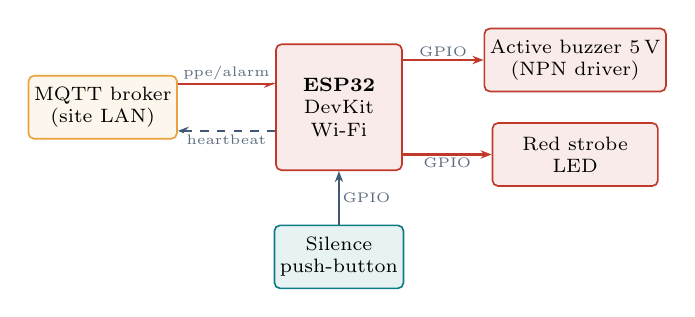
\begin{tikzpicture}
        \node[blk=amber, minimum width=1.7cm] (brk) at (0,0) {MQTT broker\\(site LAN)};
        \node[blk=crit, minimum width=1.6cm, minimum height=1.6cm] (esp) at (3.0,0) {\textbf{ESP32}\\DevKit\\Wi-Fi};
        \node[blk=crit, minimum width=2.1cm] (bz)  at (6.0, 0.6) {Active buzzer 5\,V\\(NPN driver)};
        \node[blk=crit, minimum width=2.1cm] (led) at (6.0,-0.6) {Red strobe\\LED};
        \node[blk=teal, minimum width=1.6cm] (btn) at (3.0,-1.9) {Silence\\push-button};
        \draw[arrc] ([yshift=0.3cm]brk.east) -- node[lbl, above] {ppe/alarm} ([yshift=0.3cm]esp.west);
        \draw[arr, dashed] ([yshift=-0.3cm]esp.west) -- node[lbl, below] {heartbeat} ([yshift=-0.3cm]brk.east);
        \draw[arrc] (esp.east |- bz) -- node[lbl, above] {GPIO} (bz);
        \draw[arrc] (esp.east |- led) -- node[lbl, below] {GPIO} (led);
        \draw[arr] (btn) -- node[lbl, right] {GPIO} (esp);
      \end{tikzpicture}}\par\vspace{0.6em}
      {\scriptsize Alarm message on \texttt{ppe/alarm}:\par\vspace{0.2em}
      \ttfamily \{"cmd":"on", "reason":"fire", "zone":"Z1"\}\par}
    \end{column}
    \begin{column}{0.46\textwidth}
      \scriptsize
      \textbf{\small Behaviour}
      \begin{itemize}
        \item Subscribes to \texttt{ppe/alarm} (QoS 1); fire or smoke turns on the siren and strobe.
        \item Only CRITICAL events sound the buzzer, so workers do not learn to ignore it.
        \item Silenced by the push-button or from the dashboard; turns off once the hazard clears.
      \end{itemize}
      \textbf{\small Reliability}
      \begin{itemize}
        \item Heartbeat every 5\,s plus an MQTT \emph{Last Will}~[8]; the dashboard shows
              ``alarm offline'' when it stops.
        \item Works without internet, because the broker is on the site LAN.
      \end{itemize}
      \textbf{\small Why ESP32}
      \begin{itemize}
        \item Low cost, built-in Wi-Fi, mature MQTT libraries; the Jetson stays free for inference.
      \end{itemize}
    \end{column}
  \end{columns}
\end{frame}

% =====================================================================
% 14. Event pipeline & stack
% =====================================================================
\begin{frame}{Methodology -- Event Pipeline \& Technology Stack}
  \begin{columns}[T]
    \begin{column}{0.53\textwidth}
      \small\textbf{MQTT topics}~[8]\par\vspace{0.3em}
      \scriptsize
      \renewcommand{\arraystretch}{1.25}
      \begin{tabular}{@{}l L{1.75cm} L{2.6cm}@{}}
        \toprule
        \textbf{Topic} & \textbf{From $\rightarrow$ to} & \textbf{Content}\\
        \midrule
        \texttt{ppe/alerts}    & Jetson $\rightarrow$ backend & violations, hazards, evidence path\\
        \texttt{ppe/metrics}   & Jetson $\rightarrow$ backend & rolling compliance score\\
        \texttt{ppe/heartbeat} & Jetson, ESP32 $\rightarrow$ backend & device health\\
        \texttt{ppe/alarm}     & Jetson, dashboard $\rightarrow$ ESP32 & siren on / off\\
        \bottomrule
      \end{tabular}\par\vspace{0.4em}
      Every event is JSON: type, event, priority, timestamp, worker\_id, confidence,
      compliance\_score, detections, image\_path. QoS 1, buffered on the Jetson if the network drops.
    \end{column}
    \begin{column}{0.43\textwidth}
      \small\textbf{Technology stack}\par\vspace{0.3em}
      \scriptsize
      \renewcommand{\arraystretch}{1.2}
      \begin{tabular}{@{}l L{3.5cm}@{}}
        \toprule
        Edge     & Jetson Nano, JetPack, Python, Ultralytics YOLOv8, TensorRT, OpenCV, paho-mqtt\\
        Alarm    & ESP32, Arduino framework, PubSubClient, active buzzer\\
        Messaging & Eclipse Mosquitto (MQTT)\\
        Backend  & FastAPI, PostgreSQL, WebSockets, ReportLab, pytest\\
        Frontend & React + Vite, Recharts, Tailwind CSS\\
        Tooling  & Roboflow / CVAT, PyTorch, Colab, Git, Docker\\
        \bottomrule
      \end{tabular}
    \end{column}
  \end{columns}
\end{frame}

% =====================================================================
% 15. Evaluation
% =====================================================================
\begin{frame}{Evaluation Plan}
  \begin{columns}[T]
    \begin{column}{0.56\textwidth}
      \scriptsize
      \renewcommand{\arraystretch}{1.25}
      \begin{tabular}{@{}L{3.0cm} l L{2.0cm}@{}}
        \toprule
        \textbf{Metric} & \textbf{Target} & \textbf{Method}\\
        \midrule
        mAP@0.5 (test set) {\tiny RQ1}       & $\geq$ 0.70 & Ultralytics val\\
        Per-class precision / recall          & reported    & Confusion matrix\\
        Inference speed on Jetson {\tiny RQ1} & real time   & On-device benchmark\\
        False alerts per hour {\tiny RQ2}     & debounce vs.\ none & Live session\\
        Camera $\rightarrow$ dashboard delay {\tiny RQ3} & measured & Timestamps\\
        Camera $\rightarrow$ buzzer delay {\tiny RQ3}    & $\leq$ 1\,s & Timestamps\\
        \bottomrule
      \end{tabular}
    \end{column}
    \begin{column}{0.40\textwidth}
      \small\textbf{Test scenarios}
      \begin{itemize}\scriptsize
        \item Compliant worker $\rightarrow$ green box, no alert.
        \item Helmet removed $\rightarrow$ one alert, evidence saved.
        \item Two workers, one non-compliant $\rightarrow$ per-worker result.
        \item Fire/smoke video $\rightarrow$ CRITICAL alert and \textbf{buzzer sounds}.
        \item ESP32 unplugged $\rightarrow$ ``alarm offline'' on the dashboard.
        \item Network drop $\rightarrow$ events buffered, delivered on reconnect.
      \end{itemize}
    \end{column}
  \end{columns}
\end{frame}

% =====================================================================
% 16. Work distribution
% =====================================================================
\begin{frame}{Work Distribution}
  \begin{columns}[T]
    \begin{column}{0.47\textwidth}
      \begin{block}{Uzair -- Perception}
        \small
        \begin{itemize}
          \item Dataset collection and annotation
          \item YOLOv8n training, evaluation, export
          \item Compliance engine: matching, score, debounce
          \item Evidence capture and the event handoff
        \end{itemize}
      \end{block}
    \end{column}
    \begin{column}{0.47\textwidth}
      \begin{block}{Muhammad Ahmad -- Platform}
        \small
        \begin{itemize}
          \item Jetson Nano setup and model deployment
          \item MQTT broker, publisher and backend
          \item ESP32 alarm unit: firmware and wiring
          \item Dashboard and PDF reports
        \end{itemize}
      \end{block}
    \end{column}
  \end{columns}
  \vspace{0.6em}
  \centering\small\textbf{Joint:} event format $\cdot$ integration $\cdot$ testing $\cdot$ final demo and defence
\end{frame}

% =====================================================================
% 17. Gantt
% =====================================================================
\begin{frame}{Timeline -- Gantt Chart (Two Semesters)}
  \centering
  \resizebox{\linewidth}{!}{%
  \begin{ganttchart}[
      hgrid, vgrid={*3{dotted}, {black!40, dashed}},
      x unit=0.36cm, y unit chart=0.37cm, y unit title=0.42cm,
      title height=1, title label font=\tiny\bfseries, title/.style={draw=black!50, fill=paper},
      bar height=0.55, bar/.style={draw=teal, fill=teal!70},
      bar label font=\scriptsize, group label font=\scriptsize\bfseries,
      group/.style={draw=navy, fill=navy}, group height=0.25,
      milestone/.style={fill=teal, draw=teal}, milestone label font=\scriptsize\bfseries,
      milestone height=0.5
    ]{1}{32}
    \gantttitle{FYP-I -- Fall 2026}{16}\gantttitle{FYP-II -- Spring 2027}{16}\\
    \gantttitlelist{1,...,32}{1}\\
    \ganttgroup{FYP-I}{1}{16}\\
    \ganttbar{Proposal \& literature review}{1}{4}\\
    \ganttbar{Dataset collection \& annotation}{1}{8}\\
    \ganttbar{YOLOv8n training \& evaluation}{5}{12}\\
    \ganttbar{Compliance engine}{5}{12}\\
    \ganttbar{Backend \& database}{5}{12}\\
    \ganttbar{Dashboard \& alerts}{9}{16}\\
    \ganttbar{FYP-I report \& presentation}{13}{16}\\
    \ganttgroup{FYP-II}{17}{32}\\
    \ganttbar{Jetson Nano deployment}{17}{24}\\
    \ganttbar[bar/.style={draw=crit, fill=crit!70}]{ESP32 alarm unit}{19}{24}\\
    \ganttbar{PDF reports \& integration}{21}{28}\\
    \ganttbar{System testing}{25}{32}\\
    \ganttbar{Thesis \& final demo}{29}{32}\\
    \ganttmilestone{Progress meetings}{2}
      \ganttmilestone{}{4}\ganttmilestone{}{6}\ganttmilestone{}{8}\ganttmilestone{}{10}
      \ganttmilestone{}{12}\ganttmilestone{}{14}\ganttmilestone{}{16}\ganttmilestone{}{18}
      \ganttmilestone{}{20}\ganttmilestone{}{22}\ganttmilestone{}{24}\ganttmilestone{}{26}
      \ganttmilestone{}{28}\ganttmilestone{}{30}\ganttmilestone{}{32}\\
    \ganttmilestone[milestone/.style={fill=amber, draw=amber}]{Formal reviews}{1}
      \ganttmilestone[milestone/.style={fill=amber, draw=amber}]{}{4}
      \ganttmilestone[milestone/.style={fill=amber, draw=amber}]{}{10}
      \ganttmilestone[milestone/.style={fill=amber, draw=amber}]{}{16}
      \ganttmilestone[milestone/.style={fill=amber, draw=amber}]{}{24}
      \ganttmilestone[milestone/.style={fill=crit, draw=crit}]{}{32}
  \end{ganttchart}}\par\vspace{0.2em}
  {\tiny\color{slate}
  \textcolor{teal}{$\blacksquare$} progress meeting every two weeks \quad
  \textcolor{amber}{$\blacksquare$} kickoff and formal reviews (weeks 1, 4, 10, 16, 24) \quad
  \textcolor{crit}{$\blacksquare$} final defence (week 32)\par}
\end{frame}

% =====================================================================
% 18. Meeting schedule
% =====================================================================
\begin{frame}{Timeline -- Milestones \& Supervisor Meetings}
  \small
  \renewcommand{\arraystretch}{1.3}
  \begin{tabularx}{\linewidth}{@{}l l X@{}}
    \toprule
    \textbf{Week} & \textbf{Meeting} & \textbf{Evidence shown to the supervisor}\\
    \midrule
    1  & Kickoff           & Scope agreed: worker, helmet, vest, fire, smoke\\
    4  & Proposal review   & Proposal approved; dataset sources and tools confirmed\\
    10 & Mid-term (FYP-I)  & First trained model; compliance engine running on a laptop\\
    16 & FYP-I evaluation  & Laptop demo from camera to dashboard; FYP-I report\\
    24 & Mid-term (FYP-II) & Model on the Jetson Nano; live events stored; ESP32 buzzer working\\
    32 & Final defence     & Full live demo, PDF reports, thesis and demo video\\
    \midrule
    Every 2 weeks & Progress meeting & Work done, problems, plan for the next two weeks\\
    \bottomrule
  \end{tabularx}
\end{frame}

% =====================================================================
% 19. Conclusion
% =====================================================================
\begin{frame}{Conclusion}
  \begin{columns}[T]
    \begin{column}{0.56\textwidth}
      \begin{itemize}\small
        \item PPE detection~[2,\,3] and edge fire detection~[7] are proven; real sites still lack the
              \textbf{system around the detector}.
        \item IntelliSafe adds that system: a unified edge detector, per-worker compliance with
              debounce, an MQTT event pipeline, evidence, analytics, and an \textbf{on-site ESP32
              alarm}.
        \item Success is measured on the device: mAP, FPS, false alerts per hour, and latency to the
              dashboard and to the buzzer.
      \end{itemize}
    \end{column}
    \begin{column}{0.40\textwidth}
      \begin{block}{Expected impact}
        \small
        From periodic inspection to \textbf{continuous, evidence-based} monitoring: violations are
        caught as they happen, fire is announced on site within a second, and managers see the trend
        before an accident does.
      \end{block}
    \end{column}
  \end{columns}
\end{frame}

% =====================================================================
% 20. References
% =====================================================================
\begin{frame}{References}
  \scriptsize
  \begin{enumerate}
    \item[{[1]}] International Labour Organization, \emph{A Call for Safer and Healthier Working Environments}, Geneva, 2023.
    \item[{[2]}] N.\ D.\ Nath, A.\ H.\ Behzadan, and S.\ G.\ Paal, ``Deep learning for site safety: Real-time detection of personal protective equipment,'' \emph{Automation in Construction}, vol.\ 112, 103085, 2020.
    \item[{[3]}] Z.\ Wang, Y.\ Wu, L.\ Yang, A.\ Thirunavukarasu, C.\ Evison, and Y.\ Zhao, ``Fast personal protective equipment detection for real construction sites using deep learning approaches,'' \emph{Sensors}, vol.\ 21, no.\ 10, 3478, 2021.
    \item[{[4]}] J.\ Redmon, S.\ Divvala, R.\ Girshick, and A.\ Farhadi, ``You Only Look Once: Unified, real-time object detection,'' in \emph{Proc.\ IEEE CVPR}, 2016, pp.\ 779--788.
    \item[{[5]}] G.\ Jocher, A.\ Chaurasia, and J.\ Qiu, \emph{Ultralytics YOLOv8}, 2023. \url{https://github.com/ultralytics/ultralytics}
    \item[{[6]}] NVIDIA Corporation, \emph{Jetson Nano Developer Kit}. \url{https://developer.nvidia.com/embedded/jetson-nano}
    \item[{[7]}] P.\ V.\ A.\ B.\ de Ven\^ancio, A.\ C.\ Lisboa, and A.\ V.\ Barbosa, ``An automatic fire detection system based on deep convolutional neural networks for low-power, resource-constrained devices,'' \emph{Neural Computing and Applications}, vol.\ 34, pp.\ 15349--15368, 2022.
    \item[{[8]}] OASIS, \emph{MQTT Version 5.0}, OASIS Standard, March 2019. \url{https://docs.oasis-open.org/mqtt/mqtt/v5.0/mqtt-v5.0.html}
  \end{enumerate}
\end{frame}

% =====================================================================
% 21. Thank you
% =====================================================================
\begin{frame}[plain]
  \centering
  \vspace{1.2em}
  {\Huge\bfseries\color{navy} Thank You}\par\vspace{0.4em}
  {\large\color{amber} Questions \& Discussion}\par\vspace{1.2em}
  {\color{slate!50}\rule{0.5\linewidth}{0.4pt}}\par\vspace{0.8em}
  {\normalsize\bfseries\color{navy} IntelliSafe}\par
  {\small Real-Time Working Site Safety Monitoring using Edge Computer Vision}\par\vspace{0.5em}
  {\footnotesize Muhammad Ahmad (FA23-BCE-113) $\cdot$ Uzair (FA23-BCE-098)}\par
  {\footnotesize Supervisor: Dr.\ Ikramullah Khosa}\par\vspace{0.3em}
  {\scriptsize\color{slate} Department of Computer Engineering, COMSATS University Islamabad, Lahore Campus}
\end{frame}

\end{document}
